\documentclass[../../main.tex]{subfiles}
\begin{document}

{\bf［解］}

与式を $f(x,y)$ とおく．式を少し整理すると
\begin{align}
 f(x,y) = 2\sin x + \left(\cos y + \sqrt{3}\sin y\right)\cos x
\end{align}
とかける．そこでまず$x$を固定して$y$を動かして最大最小を求めた後，$x$を動かして全体の最大最小を求める．新しく$y$に依存する部分だけを取り出して
\begin{align}
 g(y) = \cos y + \sqrt{3}\sin y
\end{align}
とおくと，コーシーシュワルツの不等式から$g(y)$は
\begin{align}
-2 \le \begin{pmatrix} 1 \\ \sqrt{3} \end{pmatrix} \cdot \begin{pmatrix} \cos y \\ \sin y \end{pmatrix} \le 2 
\end{align}
を満たす．左側の等号成立条件は
\begin{align}
 y = \frac{4\pi}{3} \label{eq:1}
\end{align}
であり，右側の等号成立条件は
\begin{align}
 y = \frac{\pi}{3} \label{eq:2}
\end{align}
である．

よって，$\cos x$の符号に応じて$x$を固定した時の$f(x,y)$の最大最小値は以下のように与えられる．
ただし三角関数の合成により
\begin{align}
\begin{cases}
 2\sin x + 2 \cos x = 2\sqrt{2}\sin\left(x+\frac{\pi}{4}\right)\\
 2\sin x - 2 \cos x = 2\sqrt{2}\sin\left(x-\frac{\pi}{4}\right)
\end{cases} 
\end{align}
と書けることを利用した．
\begin{align}
\max f(x,y) &= 
\begin{cases}
2\sqrt{2}\sin\left(x+\dfrac{\pi}{4}\right) & \left(0 \le x < \dfrac{\pi}{2}, \; \dfrac{3\pi}{2} < x \le 2\pi, y=\frac{\pi}{3} \text{ のとき}\right) \\[8pt]
2\sqrt{2}\sin\left(x-\dfrac{\pi}{4}\right) & \left(\dfrac{\pi}{2} \le x \le \dfrac{3\pi}{2}, y=\dfrac{4\pi}{3} \text{ のとき}\right)
\end{cases} \\[10pt]
\min f(x,y) &= 
\begin{cases}
2\sqrt{2}\sin\left(x-\dfrac{\pi}{4}\right) & \left(0 \le x < \dfrac{\pi}{2}, \; \dfrac{3\pi}{2} < x \le 2\pi, y=\dfrac{4\pi}{3} \text{ のとき}\right) \\[8pt]
2\sqrt{2}\sin\left(x+\dfrac{\pi}{4}\right) & \left(\dfrac{\pi}{2} \le x \le \dfrac{3\pi}{2}, y=\frac{\pi}{3} \text{ のとき}\right)
\end{cases}
\end{align}

この様子を図示すると以下のようになる．

\begin{figure}[htb]
 \begin{center}
  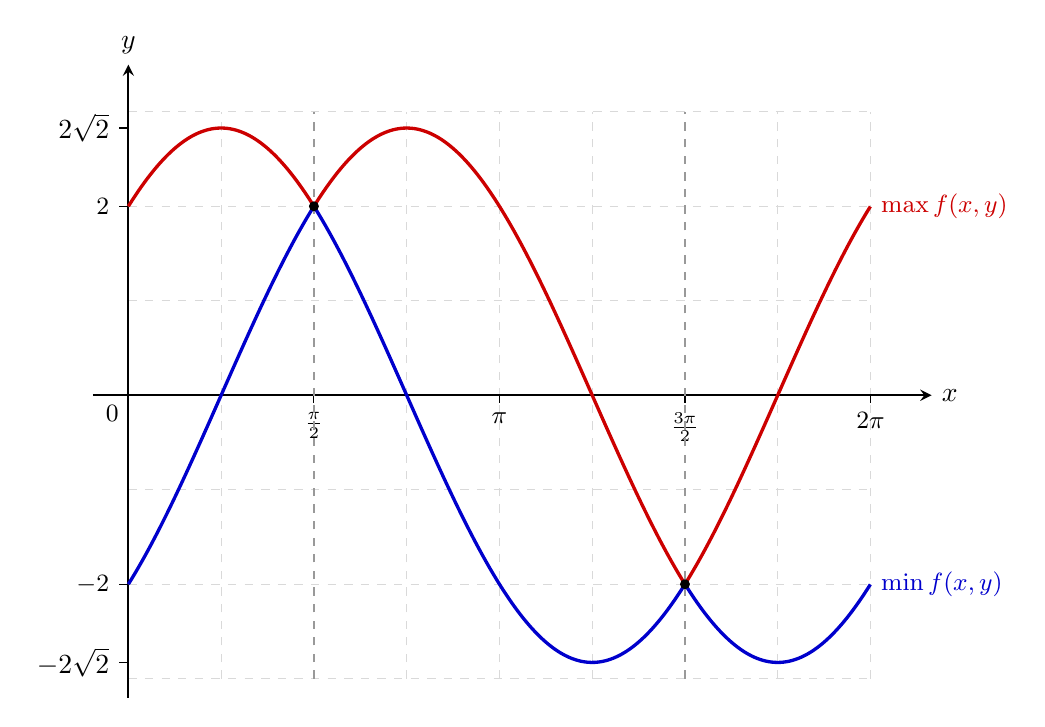
\begin{tikzpicture}[x=1.5cm, y=1.2cm, >=stealth]
    % グリッド線
    \draw[dashed, gray!30] (0,-3) grid[xstep=0.7854, ystep=1] (6.2832,3);

    % 軸の描画
    \draw[->, thick] (-0.3,0) -- (6.8,0) node[right] {$x$};
    \draw[->, thick] (0,-3.2) -- (0,3.5) node[above] {$y$};
    \node[below left, font=\small] at (0,0) {$0$};

    % y軸の目盛り
    \foreach \y in {-2, 2} {
        \draw (0,\y) -- (-0.08,\y) node[left, font=\small] {$\y$};
    }
    \draw (0, 2.828) -- (-0.08, 2.828) node[left] {$2\sqrt{2}$};
    \draw (0,-2.828) -- (-0.08,-2.828) node[left] {$-2\sqrt{2}$};

    % x軸の目盛りと境界線 (pi/2, 3pi/2)
    \foreach \x/\label in {
        1.5708/$\frac{\pi}{2}$,
        3.1416/$\pi$,
        4.7124/$\frac{3\pi}{2}$,
        6.2832/$2\pi$
    } {
        \draw (\x,0) -- (\x,-0.08) node[below, font=\small] {\label};
    }

    % cos x = 0 となる境界領域の垂直破線 (x = pi/2, x = 3pi/2)
    \draw[dashed, gray!80, thick] (1.5708, -3) -- (1.5708, 3);
    \draw[dashed, gray!80, thick] (4.7124, -3) -- (4.7124, 3);

    % -------------------------------------------------------------
    % 薄い背景曲線 (2つ全体のカーブ)
    % C1: 2*sqrt(2)*sin(x + pi/4)
    % C2: 2*sqrt(2)*sin(x - pi/4)
    % -------------------------------------------------------------
    \draw[gray!40, thin, domain=0:6.2832, samples=150, smooth]
        plot (\x, {2.828*sin((\x + pi/4) r)});
    \draw[gray!40, thin, domain=0:6.2832, samples=150, smooth]
        plot (\x, {2.828*sin((\x - pi/4) r)});

    % -------------------------------------------------------------
    % 【最大値 max f(x,y)】（赤色の太線）
    % -------------------------------------------------------------
    % (1) 0 <= x < pi/2: 2*sqrt(2)*sin(x + pi/4)
    \draw[very thick, red!80!black, domain=0:1.5708, samples=100, smooth]
        plot (\x, {2.828*sin((\x + pi/4) r)});

    % (2) pi/2 <= x < 3pi/2: 2*sqrt(2)*sin(x - pi/4)
    \draw[very thick, red!80!black, domain=1.5708:4.7124, samples=100, smooth]
        plot (\x, {2.828*sin((\x - pi/4) r)});

    % (3) 3pi/2 <= x <= 2pi: 2*sqrt(2)*sin(x + pi/4)
    \draw[very thick, red!80!black, domain=4.7124:6.2832, samples=100, smooth]
        plot (\x, {2.828*sin((\x + pi/4) r)})
        node[right, font=\small, red!80!black] {$\max f(x,y)$};

    % -------------------------------------------------------------
    % 【最小値 min f(x,y)】（青色の太線）
    % -------------------------------------------------------------
    % (1) 0 <= x < pi/2: 2*sqrt(2)*sin(x - pi/4)
    \draw[very thick, blue!80!black, domain=0:1.5708, samples=100, smooth]
        plot (\x, {2.828*sin((\x - pi/4) r)});

    % (2) pi/2 <= x < 3pi/2: 2*sqrt(2)*sin(x + pi/4)
    \draw[very thick, blue!80!black, domain=1.5708:4.7124, samples=100, smooth]
        plot (\x, {2.828*sin((\x + pi/4) r)});

    % (3) 3pi/2 <= x <= 2pi: 2*sqrt(2)*sin(x - pi/4)
    \draw[very thick, blue!80!black, domain=4.7124:6.2832, samples=100, smooth]
        plot (\x, {2.828*sin((\x - pi/4) r)})
        node[right, font=\small, blue!80!black] {$\min f(x,y)$};

    % 交点（切り替わり点）の強調プロット
    \fill[black] (1.5708, 2) circle (1.8pt);
    \fill[black] (4.7124, -2) circle (1.8pt);

\end{tikzpicture}
\caption{$f$の最大最小の様子．}
 \end{center}
\end{figure}


従って最大最小を与える$x,y$は以下のようにまとめられる．
\begin{align}
\begin{cases}
\max f = 2\sqrt{2} & \left( (x,y) = \left(\frac{\pi}{4}, \frac{\pi}{3}\right), \left(\frac{3}{4}\pi, \frac{4}{3}\pi\right) \right) \\[1ex]
\min f = -2\sqrt{2} & \left( (x,y) = \left(\frac{5}{4}\pi, \frac{\pi}{3}\right), \left(\frac{7}{4}\pi, \frac{4}{3}\pi\right) \right)
\end{cases} 
\end{align}
\newpage

\end{document}
